\section{3D Rekonstruktion}
\subsection{Tool Ökosystem}
\subsubsection{3D Datenverarbeitung}
Als zentrales Werkzeug zur Verarbeitung dreidimensionaler Informationen wurde die Pointcloud Library (PCL) \footnote{\url{http://www.poindclouds.org}} aufgrund von vorhandenen Vorkenntnissen aus vorigen Arbeiten ausgewählt. PCL ist ein umfangreiches OpenSource C++ Framework zur Verarbeitung von Punktwolken. In mehreren Bibliotheksmodulen bietet PCL Implementierungen von gängigen Algorithmen zur Verarbeitung von räumlichen Informationen.\\
PCL selber verwendet ein Anzahl gängiger Bibliotheken zur Datenrepräsentation und -verarbeitung:

\begin{itemize}
		\item Boost 1.55 \footnote{\url{http://www.boost.org}} - für Shared Pointer
		\item Eigen3 \footnote{\url{http://eigen.tuxfamily.org}} - Matrizen, Vektoren, Lineare Algebra
		\item flann \footnote{\url{http://www.cs.ubc.ca/research/flann/}} - Fast Library for Approximate Nearest Neighbours
		\item Qt \footnote{\url{http://qt-project.org/}}- GUI Framework
		\item vtk 6.1 \footnote{\url{http://www.vtk.org/}} - Visualization ToolKit
		\item qHull \footnote{\url{http://www.qhull.org/}} - Triangulation (Convex/Concave Hull, Delaunay, Voronoi usw.)
		\item OpenNI2 \footnote{\url{http://structure.io/openni}} - zur Einbindung OpenNI-kompatibler Sensoren
		\item CUDA \footnote{\url{https://developer.nvidia.com/about-cuda}} - für GPU Implementierungen verschiedener Algorithmen
\end{itemize}

Diese Vielzahl von Abhängigkeiten sowie der Entwicklungszyklus von PCL haben einen großen Anteil am Aufwand zum Aufsetzen der Produktionsumgebung. Da vor allem die GPU-beschleunigten Verfahren sowie die Einbindung neuerer OpenNI2-kompatibler Sensoren noch nicht im neuesten Release eingebunden sind, ist die eigene Kompilierung der Bibliothek im aktuellen Stand der Entwicklung erforderlich. Im Laufe der Projekt 1 Veranstaltung wurde dies teilweise am tagesaktuellen Entwicklungsstand von PCL durchgeführt.

\subsubsection{Visualisierung}
Um zunächst losgelöst von der Unity-basierten \footnote{\url{http://unity3d.com/}} Visualisierungskomponente des I$^2$E-Projekts eine Visualisierungslösung nutzen zu können, wurde ein lokales Userinterface entwickelt, welches auf openFrameworks \footnote{\url{http://openframeworks.cc}} basiert. Dieses wird über das Signal-Slot System von Boost an die 3D Verarbeitung angebunden, um Parameter von Punkt- und Meshprozessoren zur Laufzeit zu verändern und Zwischenergebnisse und das Resultat der Rekonstruktion zu visualisieren. Für Steuerelemente im Userinterface werden die openFrameworks Erweiterungen ofxUI \footnote{\url{https://github.com/rezaali/ofxUI}} und ofxXmlSettings \footnote{\url{http://www.openframeworks.cc/documentation/ofxXmlSettings/ofxXmlSettings.html}} verwendet. Weiterhin werden die Erweiterungen ofxMSATimer \footnote{\url{https://github.com/memo/ofxMSATimer}} und ofxTimeMeasurements \footnote{\url{https://github.com/armadillu/ofxTimeMeasurements}} verwendet um dem Zeitbedarf einzelner Schritte messen zu können.

\subsection{Architektur}
Die Kernfunktionalität der User-Rekonstruktion wird in der Bibliothek \textit{libdynrecon} implementiert, welche nur Abhängigkeiten zur PCL Biliothek und deren Abhängigkeiten besitzt.

\subsubsection{Sensoranbindung}
Die Daten verschiedener Sensoren werden über ein gemeinsames Interface entgegengenommen. Hierfür wurde die abstrakte Klasse \textit{AbstractPointCloudGenerator} (siehe Abbildung \ref{fig:classdiag}) entworfen, die eine PointCloud bereitstellt. Da damit gerechnet werden muss, dass eine angebundene Sensorkomponente in einem eigenen Thread laufen kann, wird der Zugriff auf die produzierte PointCloud mittels Mutex geschützt. Die letzte PointCloud wird in einer separaten Variable gespeichert, damit im Falle einer Lock-Kollision von Generator und Konsumententhread trotzdem nicht-blockierend eine PointCloud geliefert werden kann.\\

Im Moment ist mit \textit{PclOpenNI2Grabber} (siehe Abbildung \ref{fig:classdiag}) eine Implementation vorhanden, welche den in PCL implementierten OpenNI2Grabber verwendet. Mit dieser Implementierung können OpenNI2-kompatible Sensoren wie die Microsoft XBOX Kinect, Primesense Carmine oder Asus Xtion verwendet werden.\\

Als Erweiterung ist hier zunächst ein PointCloudGenerator geplant, welcher allgemein Tiefenbilder in Punktwolken umwandeln kann. Dieser Schritt vereinfacht die zukünftige Einbindung verschiedener Sensoren die solch ein Tiefenbild liefern können. Unter anderem soll damit die Anbindung von Microsoft Kinect2SDK kompatibler Sensoren realisiert werden.

\subsubsection{3D Datenverarbeitung}
Die Verarbeitung der Sensordaten zu Polygonmeshes wird generell in einer Pipeline realisiert. Dafür werden verschiedene Punkt- und Meshprozessoren definiert, die in unterschiedlicher Weise kombiniert werden können. Punktprozessoren nehmen eine Punktwolke entgegen, und liefern eine modifizierte Punktwolke zurück. Meshprozessoren nehmen ebenso eine Punktwolke entgegen, produzieren aber ein PolygonMesh. Um dies abzubilden wurden die abstrakten Klassen \textit{AbstractProcessingPipeline}, \textit{AbstractPointProcessor} und \textit{AbstractMeshProzessor} entworfen (siehe Abbildung \ref{fig:classdiag}).\\

Im Moment existiert eine implementierte Pipeline (\textit{Pipeline01}) welche aus einem \textit{DepthThreshold} Punktprozessor und einem \textit{OrganizedFastMeshProcessor} Meshprozessor besteht. Mit Hilfe des Punktprozessors wird der weiterzuverarbeitende Tiefenbereich eingegrenzt. Der Tiefenbereich wird durch einen Minimal- und Maximalwert definiert, und Punkte außerhalb dieses Intervalls werden verworfen. Hierdurch wird eine ausreichend gute Segmentierung des Benutzers vom Hinter- und Vordergrund erreicht. Die so gefilterte Pointcloud wird an den Meshprozessor weitergegeben. Der \textit{OrganizedFastMeshProcessor} nutzt nun die Tatsache, dass die Punktwolke aus einem Tiefenbild entstanden ist, und somit organisiert ist. Das bedeutet, dass zu jedem Punkt die Nachbarpunkte wohlbekannt sind. Mit einer definierbaren Schrittweite werden aus in X-Y Ebene benachbarte Punkte zu Dreiecken verbunden. Diese Dreiecke werden dann als Vektoren aus Punktindizes geliefert, welche im Moment direkt zu Erzeugung eines openFrameworks Polygonmeshes genutzt werden. Diese Umwandlung ist momentan verantwortlich für die letzte verbliebene Abhängigkeit der Rekonstruktionsbibliothek von openFrameworks, welche in der weiteren Entwicklung ausgelagert werden wird.\\

In Zukunft sollen weitere Punkt- und Meshprozessoren implementiert werden, um mit ihnen verschiedene Pipelines aufzubauen und gegeneinander evaluieren zu können. Dazu wird die oben beschriebene Architektur vermutlich noch einige Anpassungen erfahren. Es zeichnet sich zum Beispiel die Notwendigkeit einer weiteren abstrakten Prozessor-Klasse zum Mesh Postprocessing ab. Über diese Klasse könnten dann Nachbearbeitungsschritte wie zum Beispiel Mesh-Glättung realisiert werden.


\subsection{Zukünftige Entwicklung}
\subsubsection{Einbindung mehrerer Sensoren}
Damit die Daten mehrerer Sensoren parallel erfasst werden können ist die Realisierung einer Sensor Management Komponente geplant. Diese soll sich um die Synchronisierung der eingehenden Daten kümmern sowie die Transformation der Daten in ein gemeinsames Koordinatensystem übernehmen.

\subsubsection{Kalibrierung}
Für die Überführung der Daten verschiedener Sensoren in ein gemeinsames Koordinatensystem ist die Implementierung eines Kamerakalibrierungsverfahrens erforderlich. Geplant ist hier ein möglichst automatisches Verfahren, welches aus Korrespondenzen in den Punktwolken der einzelnen Sensoren Transformationsparameter für die Daten jedes Sensors berechnet. Diese Korrespondenzen könnten zum Beispiel über die Erkennung dreidimensionaler Objekte in den Punktwolken gefunden werden.

\subsubsection{Mesh-Streaming}
Damit ein rekonstruiertes Mesh auch auf der zentralen Visualisierungskomponente der Projektanwendung dargestellt werden können, muss das Mesh über die Netzwerkkomponente serialisiert und gestreamt werden. Hierfür wird zunächst die C++ Implementierung des Netzwerkadapters fertiggestellt, auf den noch in Kapitel \ref{sec:network} eingegangen wird. Danach muss zunächst getestet werden ob sich die geplante Netzwerk Architektur der Gesamtanwendung auch für das Streaming von Polygonmeshes eignet, oder ob hierfür eine separate Lösung gefunden werden muss.

\onecolumn

\begin{figure}[h]
	\begin{center}		
		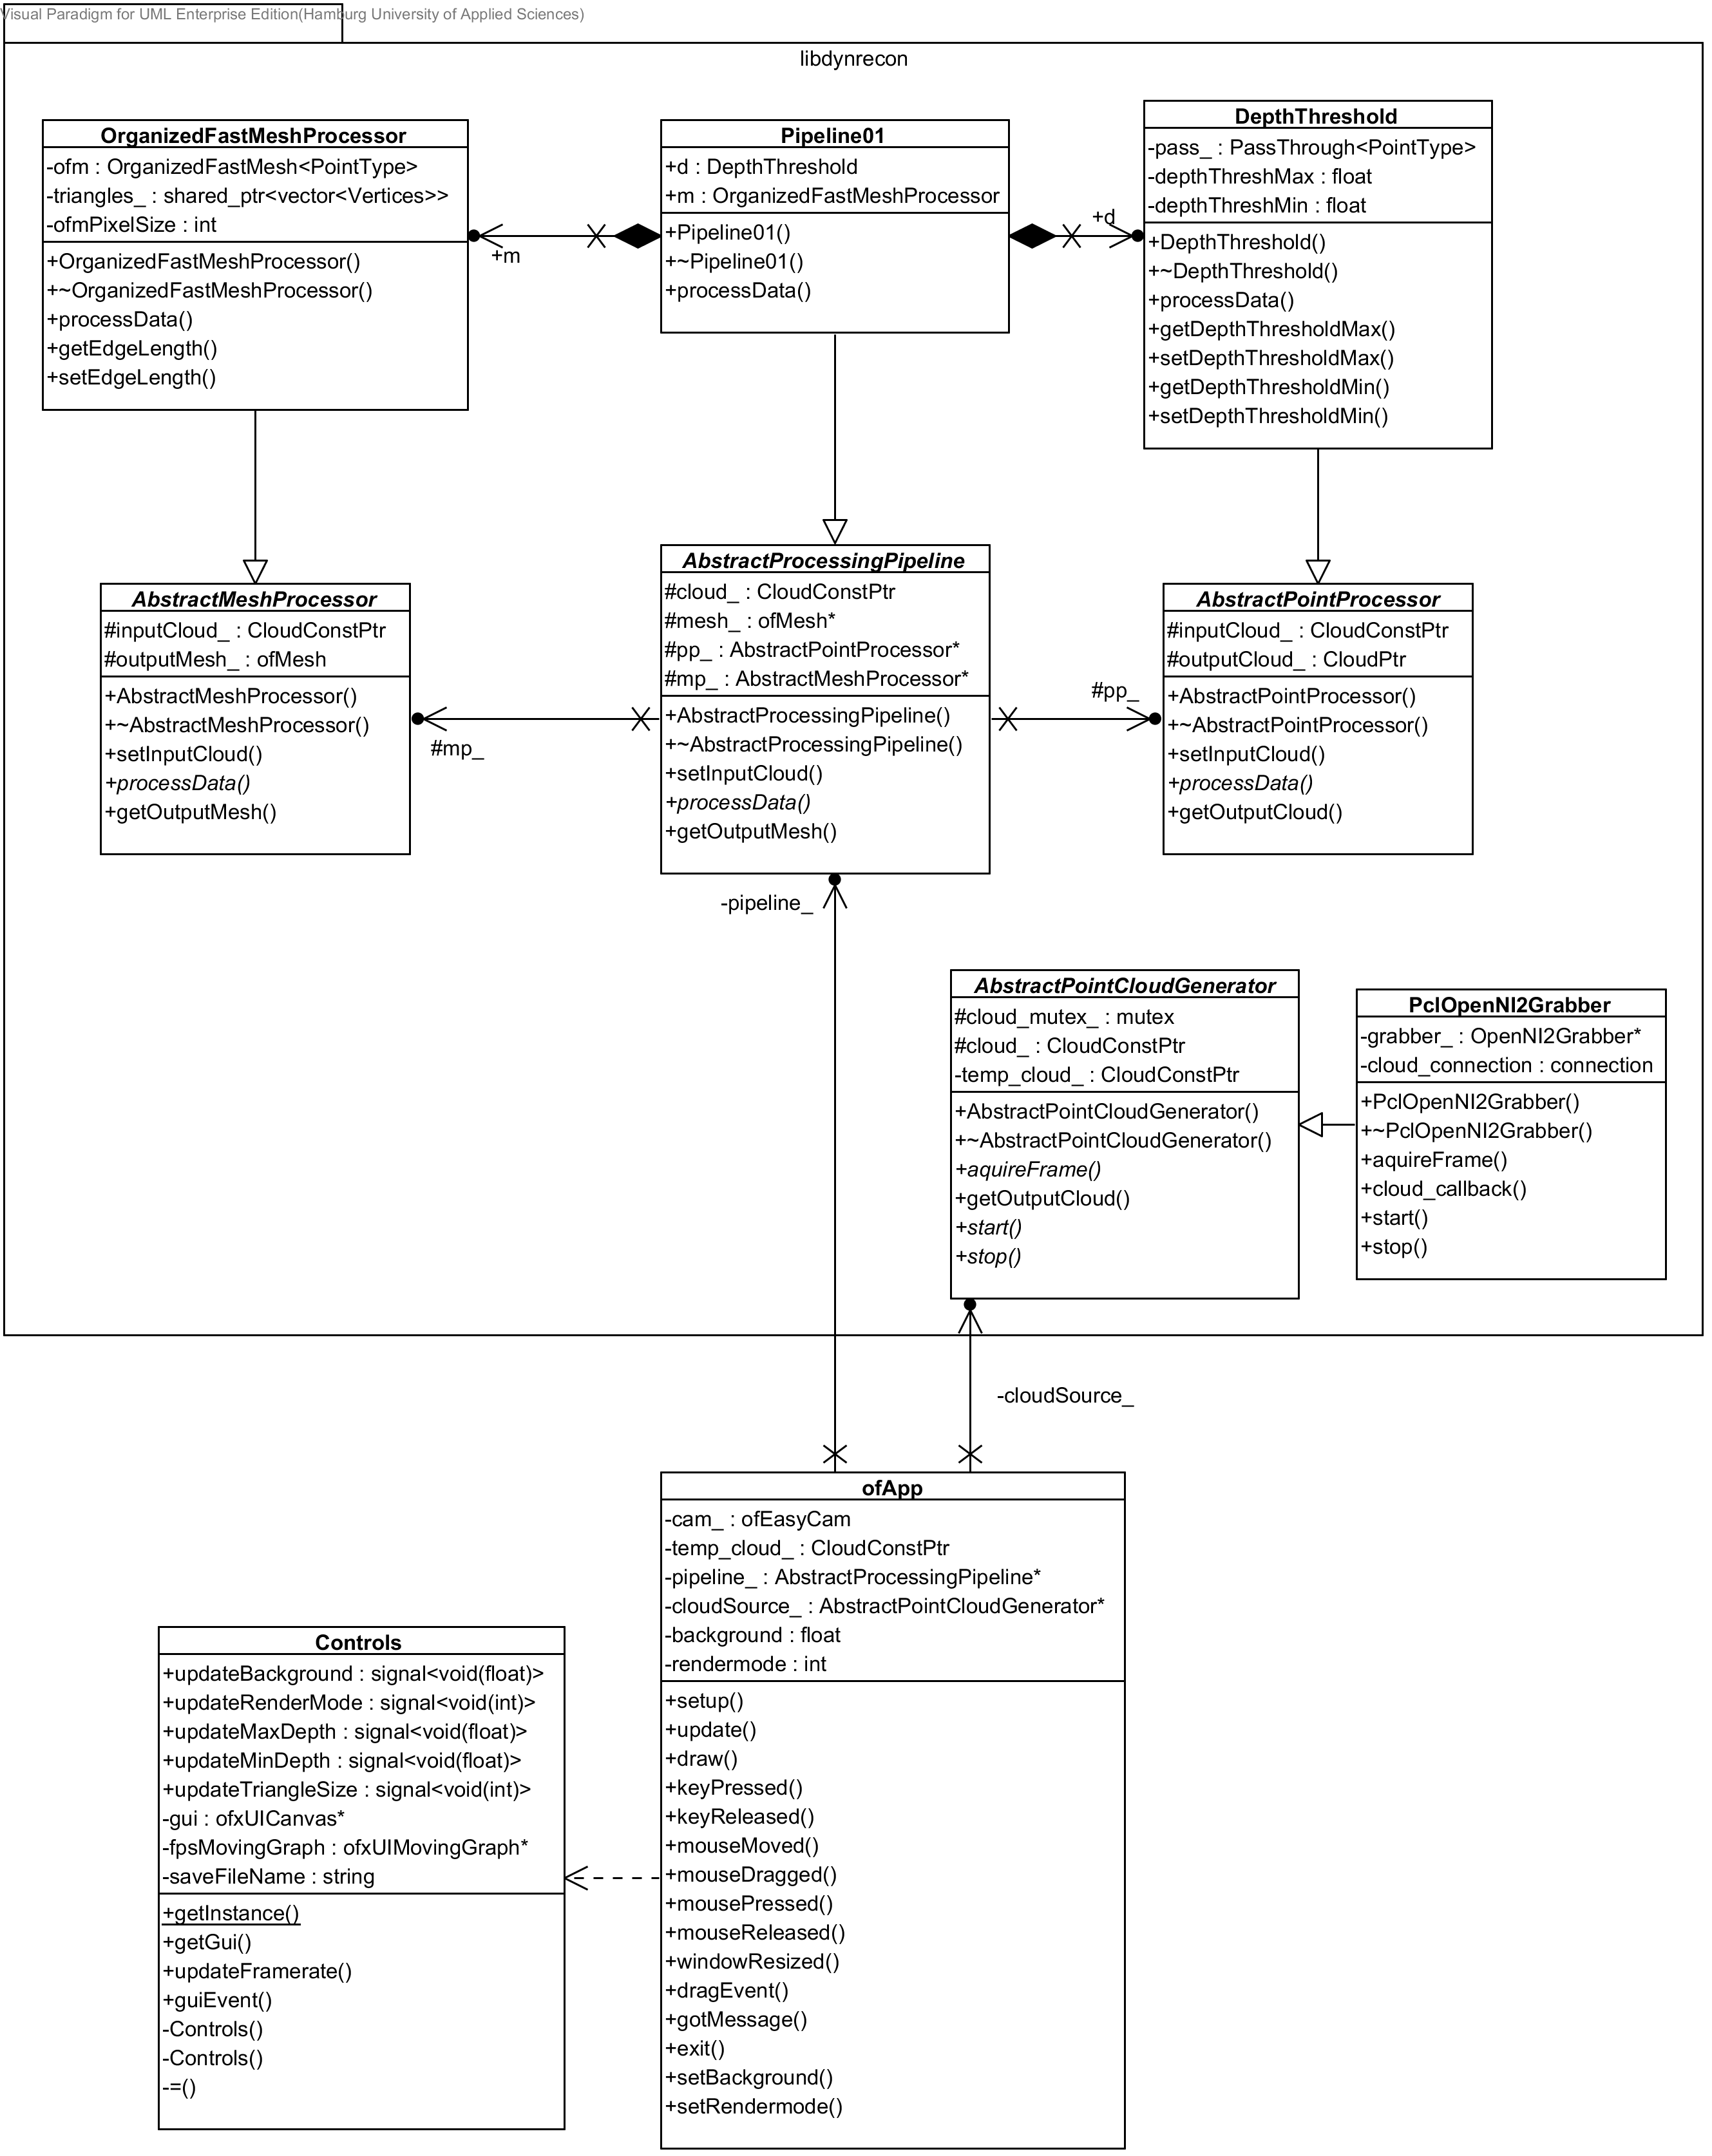
\includegraphics[width=\textwidth, keepaspectratio]{img/class_diagram}
		\caption{Klassen Diagramm der User-Reconstruction Komponente}
		\label{fig:classdiag}
	\end{center}
\end{figure}

\twocolumn
